% 03-results-and-discussions.tex

% Section Title
\section{RESULTS AND DISCUSSIONS} \label{sec:results}

    \subsection{Baseline Performance: Static vs.\ Dynamic}

        Comparing the static and dynamic scenarios highlights key differences in GNSS signal behavior, measurement stability, and receiver performance. 
        Although both datasets were collected under similar atmospheric conditions, the receiver's motion in the dynamic case introduced visible changes across all GNSS indicators.
    
        \vspace{0.5em}
        \textbf{Pseudoranges vs Time.} 
        In the static case, pseudorange lines are mostly flat with occasional steps, reflecting steady satellite tracking and minimal receiver movement. 
        In contrast, the dynamic case presents more pronounced variations, including jumps and slight trends, consistent with the receiver's motion on the Tram 15 route. 
        SV 12 and SV 25 in particular show transient signal loss or handover events. 
        These fluctuations reflect changes in satellite geometry and potential occlusions caused by urban structures.
        
        \begin{figure}[h!]
            \centering
            \begin{subfigure}{0.23\textwidth}
                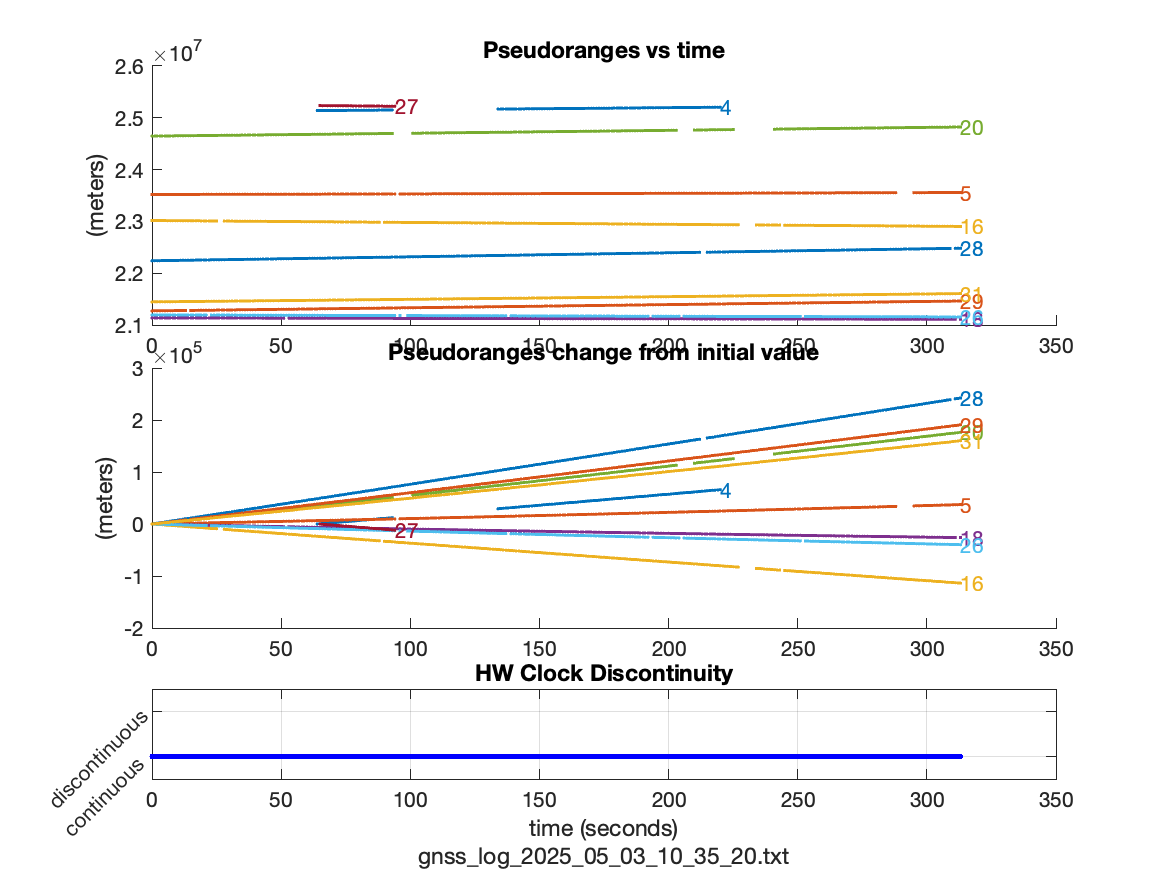
\includegraphics[width=\textwidth]{images/tests/Monte_Cappuccini/png/Samsung_A51_Monte_Cappuccini_fig1.png}
                \caption{Static: Pseudoranges vs time}
            \end{subfigure}
            \hfill
            \begin{subfigure}{0.23\textwidth}
                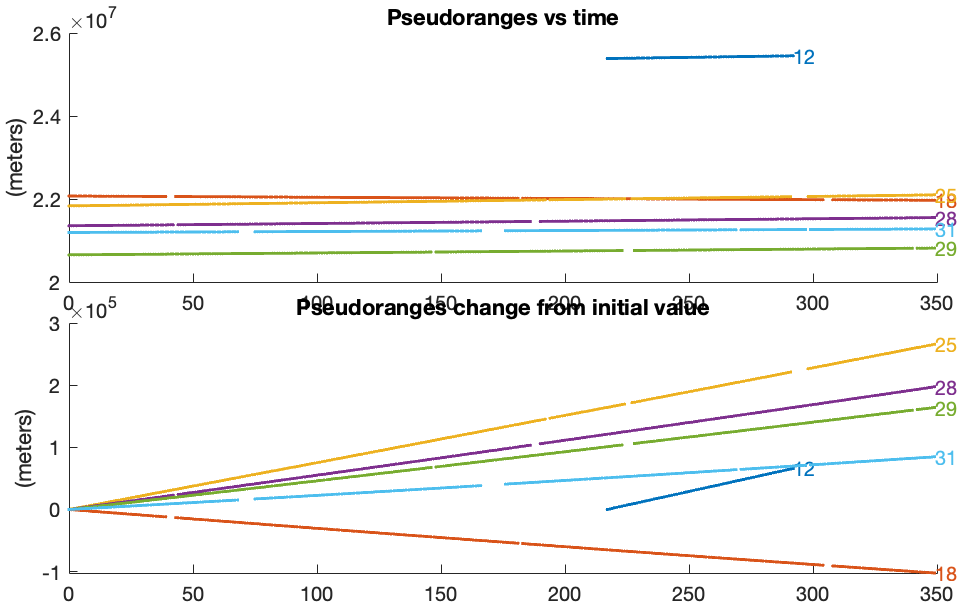
\includegraphics[width=\textwidth]{images/tests/Tram_15_trip_Castello_to_Pescatore/filtered/Samsung_A51_Tram_15_trip_Castello_to_Pescatore_fig1.png}
                \caption{Dynamic: Pseudoranges vs time}
            \end{subfigure}
        \end{figure}
    
        \vspace{0.5em}
        \textbf{Pseudorange Change from Initial Value.} 
        The static dataset showed modest drifts in pseudoranges, largely attributable to receiver clock drift. 
        The dynamic scenario, however, featured distinct upward and downward trends for different satellites (e.g., SV 25 increasing, SV 18 decreasing), corresponding to the receiver's motion relative to each satellite. 
        This behavior confirms continuous positional change and introduces measurement dynamics absent in the static case.
    
        \begin{figure}[H]
            \centering
            \begin{subfigure}{0.23\textwidth}
                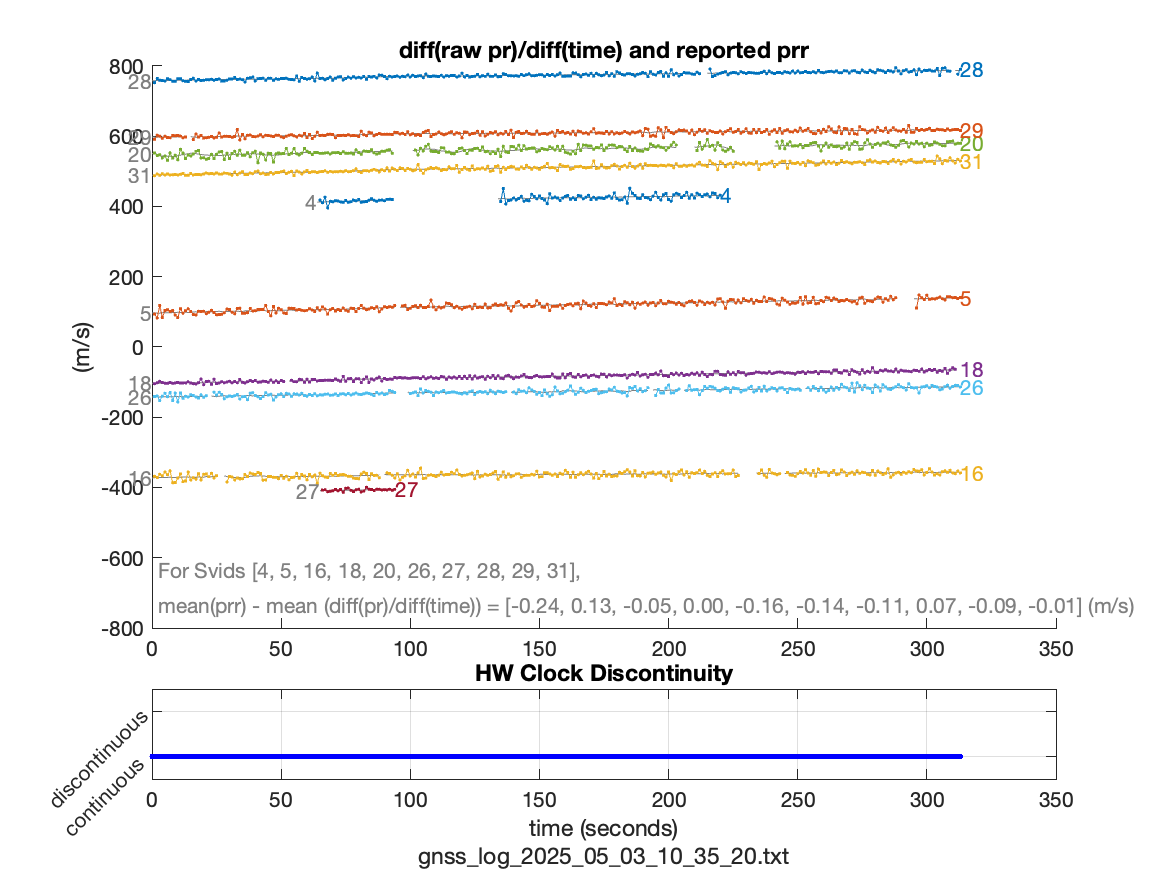
\includegraphics[width=\textwidth]{images/tests/Monte_Cappuccini/png/Samsung_A51_Monte_Cappuccini_fig2.png}
                \caption{Static: $\Delta$ Pseudorange}
            \end{subfigure}
            \hfill
            \begin{subfigure}{0.23\textwidth}
                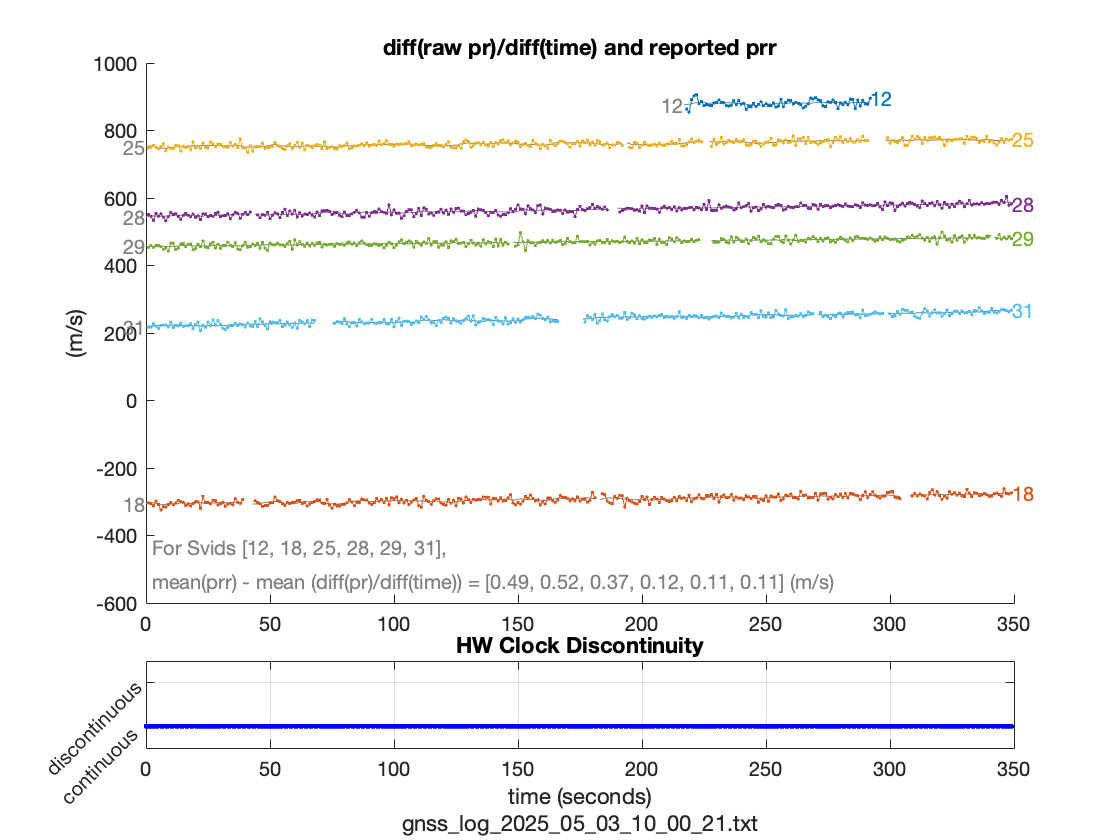
\includegraphics[width=\textwidth]{images/tests/Tram_15_trip_Castello_to_Pescatore/filtered/Samsung_A51_Tram_15_trip_Castello_to_Pescatore_fig2.png}
                \caption{Dynamic: $\Delta$ Pseudorange}
            \end{subfigure}
        \end{figure}
    
        \vspace{0.5em}
        \textbf{Positioning and Speed.} 
        The position scatter in the static case remains tightly clustered, with near-zero horizontal speed, while the dynamic dataset exhibits a more dispersed cloud with higher velocity peaks (up to 20 m/s). 
        These variations reflect real movement and acceleration events captured during Tram 15 trip from Piazza Castello to Piazza Vittorio Veneto. 
        HDOP is comparably low in both scenarios, although it exhibits more fluctuation in the dynamic case, due to changing satellite visibility and geometry.
    
        \begin{figure}[h!]
            \centering
            \begin{subfigure}{0.23\textwidth}
                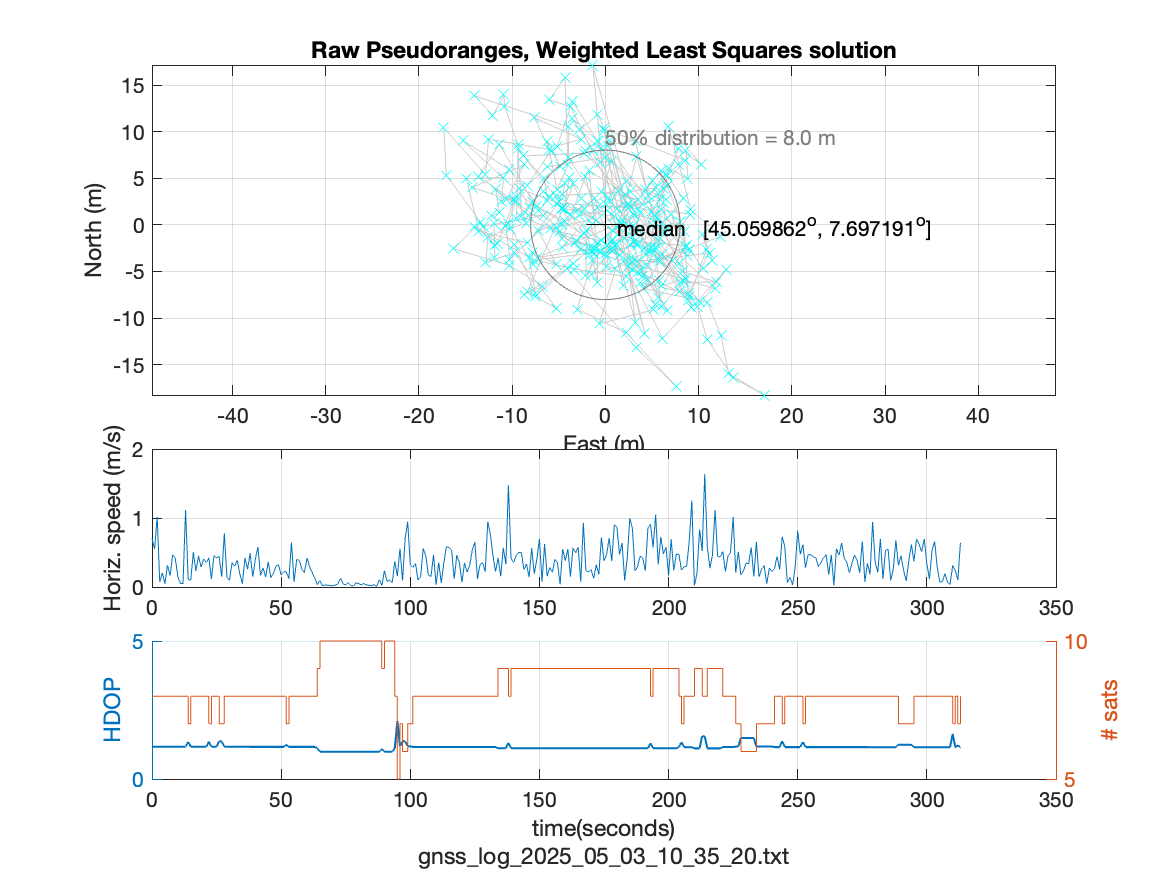
\includegraphics[width=\textwidth]{images/tests/Monte_Cappuccini/png/Samsung_A51_Monte_Cappuccini_fig4.png}
                \caption{Static: Position, Speed, HDOP}
            \end{subfigure}
            \hfill
            \begin{subfigure}{0.23\textwidth}
                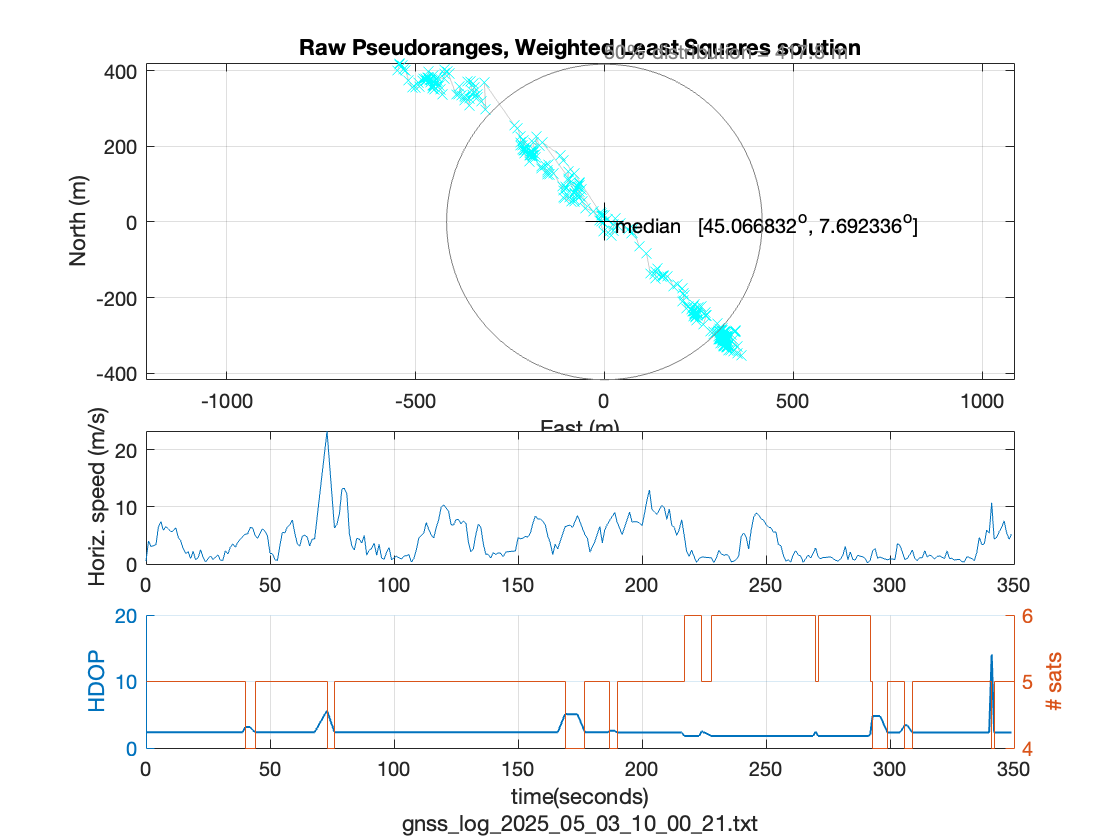
\includegraphics[width=\textwidth]{images/tests/Tram_15_trip_Castello_to_Pescatore/filtered/Samsung_A51_Tram_15_trip_Castello_to_Pescatore_fig4.png}
                \caption{Dynamic: Position, Speed, HDOP}
            \end{subfigure}
        \end{figure}
    
        \vspace{0.5em}
        \textbf{State Offsets and Timing Bias.} 
        The static clock bias grows linearly, indicating thermal-induced drift. 
        The dynamic scenario shows similar behavior, but with slightly more noise in the frequency offset and position offsets due to motion and rapid changes in the Doppler environment. 
        Despite this, both datasets show eventual stabilization, suggesting effective internal correction mechanisms.
    
        \begin{figure}[h!]
            \centering
            \begin{subfigure}{0.23\textwidth}
                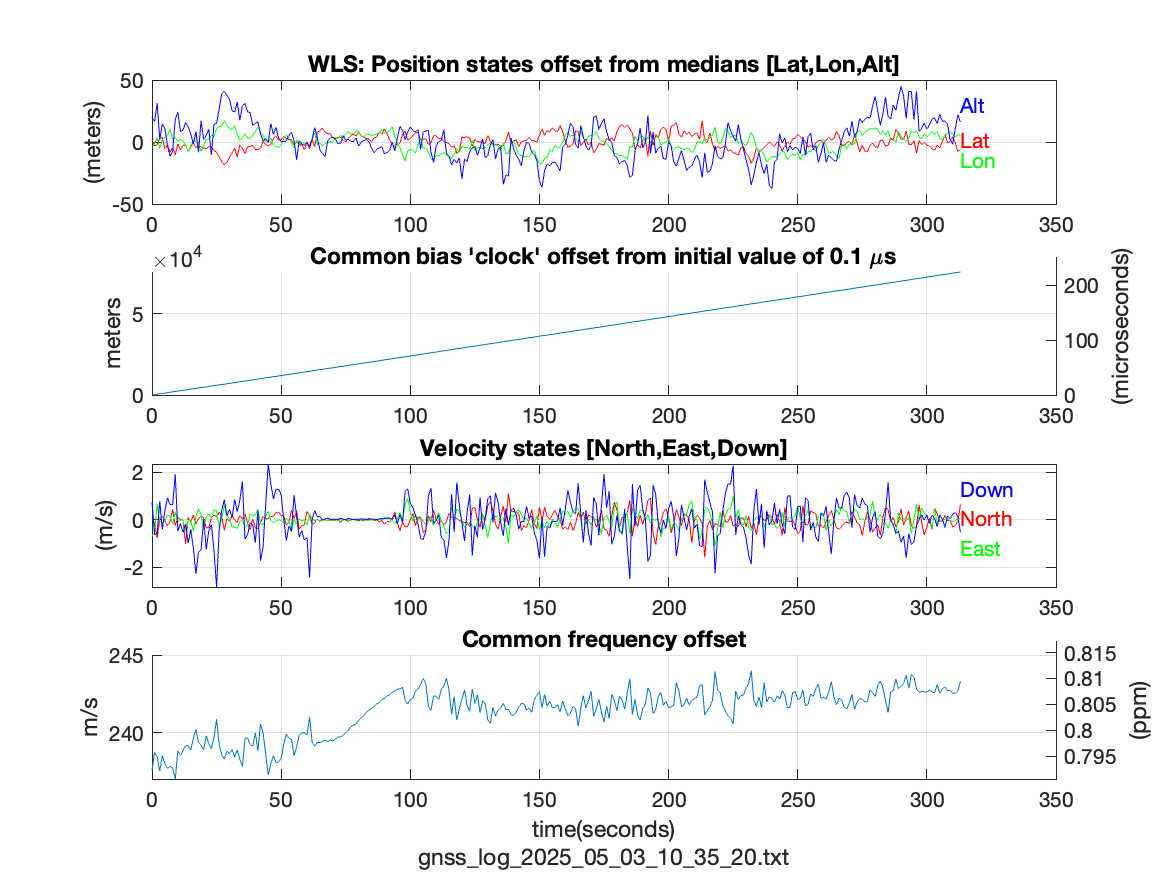
\includegraphics[width=\textwidth]{images/tests/Monte_Cappuccini/png/Samsung_A51_Monte_Cappuccini_fig5.png}
                \caption{Static: WLS states and bias}
            \end{subfigure}
            \hfill
            \begin{subfigure}{0.23\textwidth}
                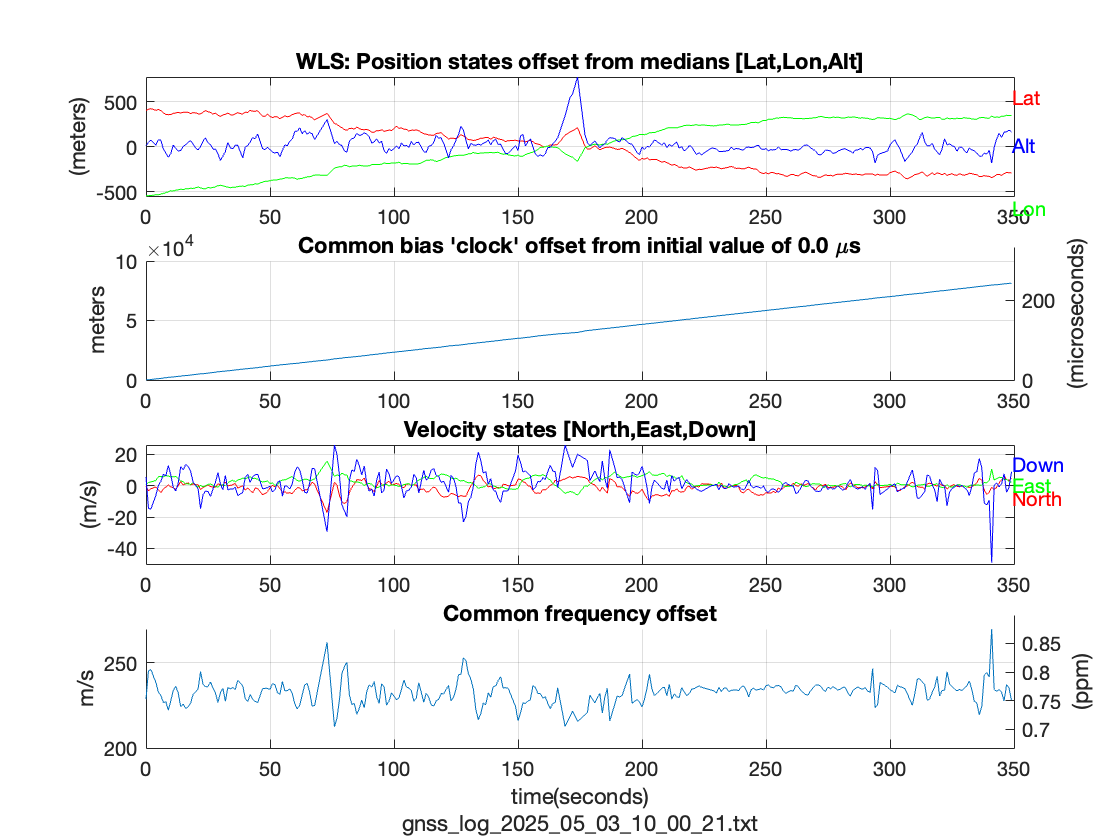
\includegraphics[width=\textwidth]{images/tests/Tram_15_trip_Castello_to_Pescatore/filtered/Samsung_A51_Tram_15_trip_Castello_to_Pescatore_fig5.png}
                \caption{Dynamic: WLS states and bias}
            \end{subfigure}
        \end{figure}
    
        \vspace{0.5em}
        \noindent Overall, the dynamic dataset reveals the expected effects of motion on GNSS signals—greater variability, signal interruptions, and increased velocity states. 
        In contrast, the static case offers a stable baseline, essential for identifying anomalies and for future spoofing detection tasks.

    \subsection{Impact of Spoofed Position}

        In a spoofing attack, counterfeit signals are broadcast to mimic GNSS transmissions, often altering their timing, amplitude, or content. 
        Typically, these deceptive signals are sent at higher power than the originals to mislead navigation systems. 
        In our experiment, however, spoofing was implemented purely in software by adjusting the perceived reception time inside the professor’s script to simulate spoofing behavior.
            
        \noindent For the spoofed test we manually injected the coordinates of Piazza Vittorio Veneto (45.064749246294085, 7.6954660899754215) — a location adjacent to our true survey point — directly into the processing script. 
        As shown in the “Spoofed Case” plots (see attached PDF), this causes the solver to converge exactly at the Piazza Vittorio Veneto coordinates rather than the true measurement site, introducing a horizontal displacement of several hundred metres.
        
        \noindent Despite this spatial shift, all raw observables remain essentially unchanged relative to the normal run:
        
        \begin{itemize}
            \item \textbf{Carrier-to-noise density (C/N):} Histograms and time-series trace exactly overlap those of the baseline, confirming no change in received signal strength.
            \item \textbf{Dilution of precision (PDOP):} The satellite geometry quality curve is identical, indicating unchanged constellation geometry.
            \item \textbf{Pseudorange residuals:} The overall spread remains the same, but the entire residual distribution is offset by the constant delay corresponding to the spoofed displacement.
        \end{itemize}

        \begin{figure}[h!]
            \centering
            \begin{subfigure}{0.23\textwidth}
                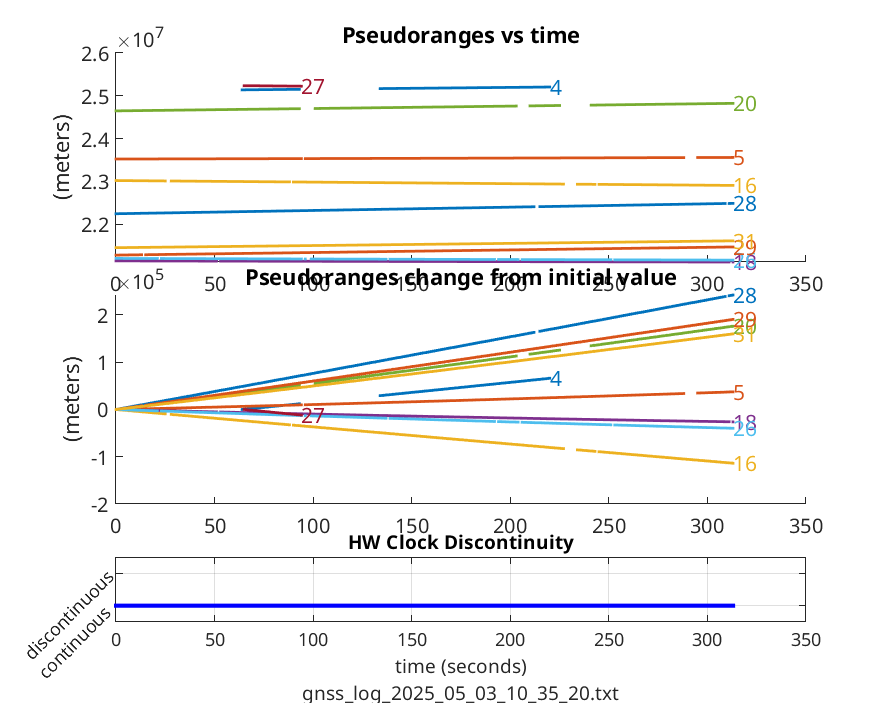
\includegraphics[width=\textwidth]{images/tests/Monte_Cappuccini/Spoofing/task5_figures/Samsung_A51_Monte_Cappuccini_fig1.png}
                \caption{Spoofed: Pseudoranges vs time}
            \end{subfigure}
            \hfill
            \begin{subfigure}{0.23\textwidth}
                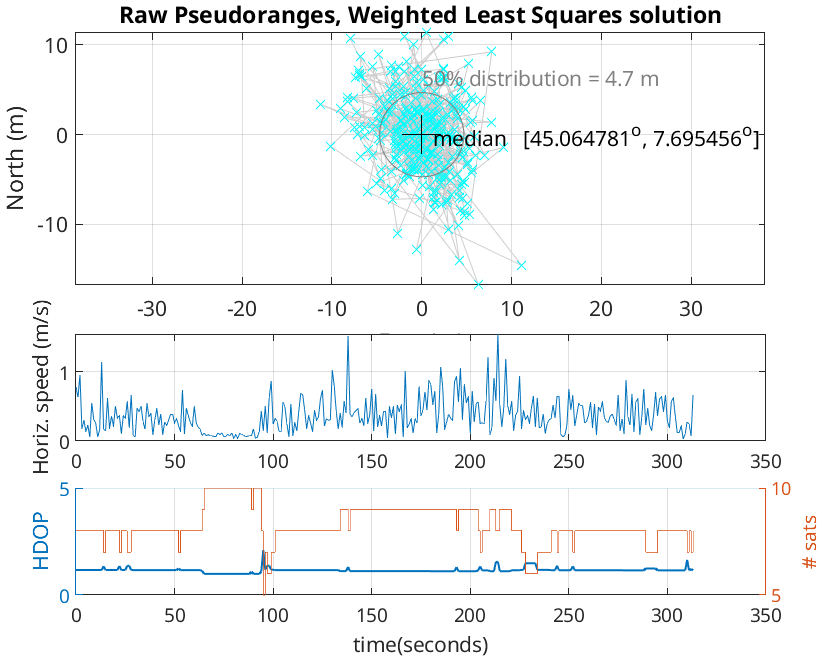
\includegraphics[width=\textwidth]{images/tests/Monte_Cappuccini/Spoofing/task5_figures/Samsung_A51_Monte_Cappuccini_fig4.png}
                \caption{Spoofed: Position, Speed, HDOP}
            \end{subfigure}
        \end{figure}


        \begin{figure}[h!]
            \centering
            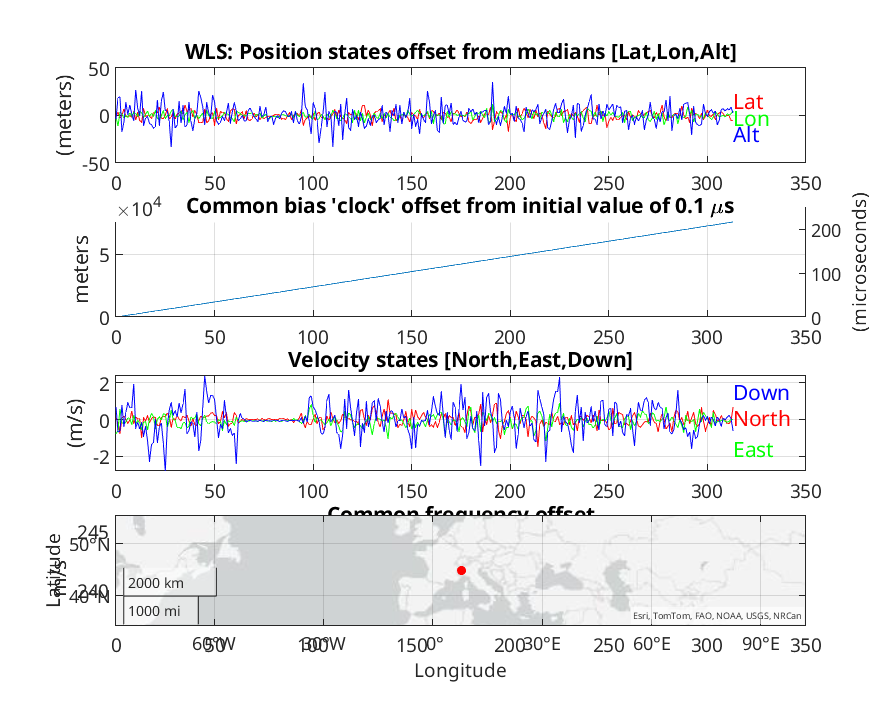
\includegraphics[width=0.9\columnwidth]{images/tests/Monte_Cappuccini/Spoofing/task5_figures/Samsung_A51_Monte_Cappuccini_fig5.png}
            \caption{Spoofed: WLS states and bias}
        \end{figure}

        
        \noindent Additionally, the 50\% (interquartile) range in the median-error distribution shrinks from approximately 8 m in the genuine case to about 4.7 m under spoofing. 
        This reduction occurs because the solver consistently “locks” onto the spoofed coordinate, decreasing variability around that false point.

    \subsection{Effects of Timing Delays}

        In this delayed-spoofing scenario we again target the same true survey point but now introduce a software-only replay delay: the spoofer “listens” to genuine signals, waits 1 ms, then injects the spoofed Piazza Vittorio Veneto coordinates starting at 50 s into the run. 
        The key parameters are set as:

        \begin{verbatim}
cfg.delay   = 1e-3;
cfg.t_start = 50;
        \end{verbatim}


        \begin{figure}[h!]
            \centering
            \begin{subfigure}{0.23\textwidth}
                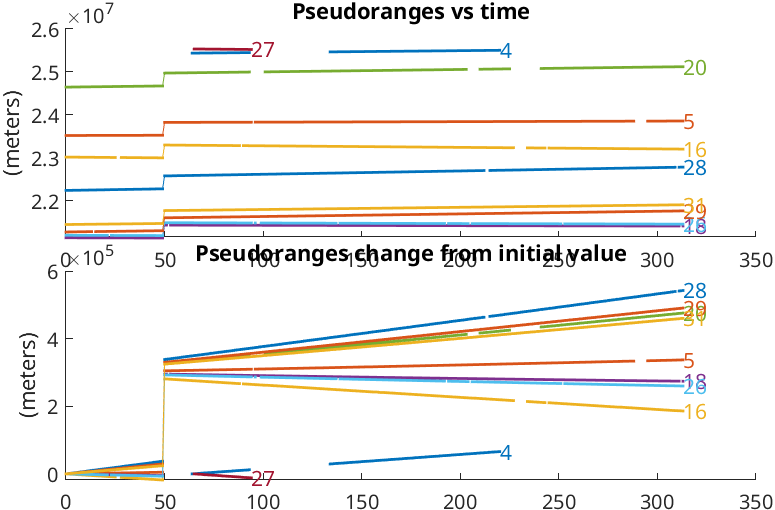
\includegraphics[width=\textwidth]{images/tests/Monte_Cappuccini/Spoofing/task6_figures/Samsung_A51_Monte_Cappuccini_fig1.png}
                \caption{Delay: Pseudoranges vs time}
            \end{subfigure}
            \hfill
            \begin{subfigure}{0.23\textwidth}
                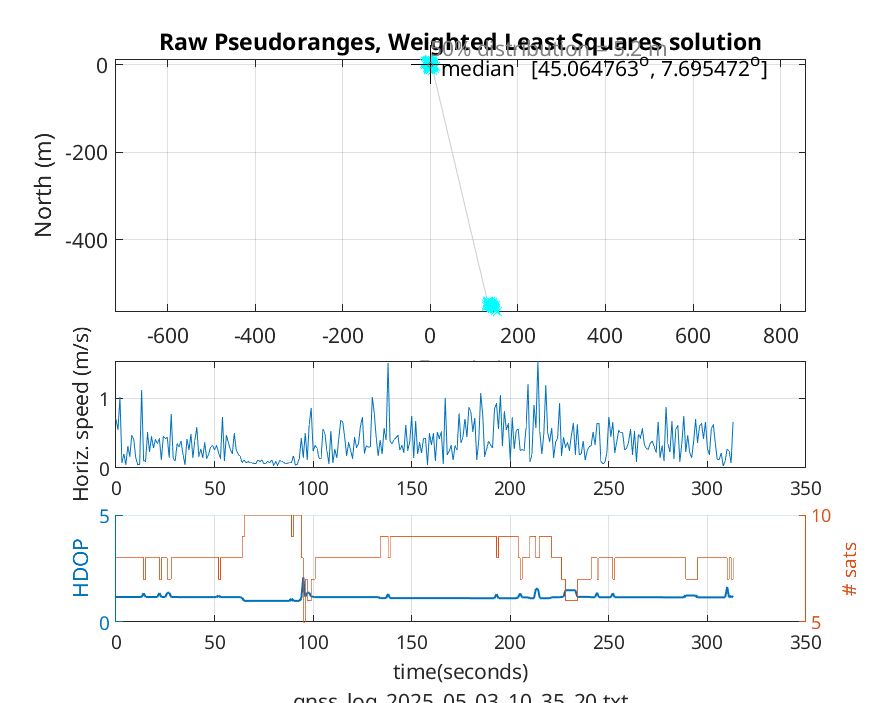
\includegraphics[width=\textwidth]{images/tests/Monte_Cappuccini/Spoofing/task6_figures/Samsung_A51_Monte_Cappuccini_fig4.png}
                \caption{Delay: Position, Speed, HDOP}
            \end{subfigure}
        \end{figure}

                \begin{figure}[h!]
            \centering
            \begin{subfigure}{0.23\textwidth}
                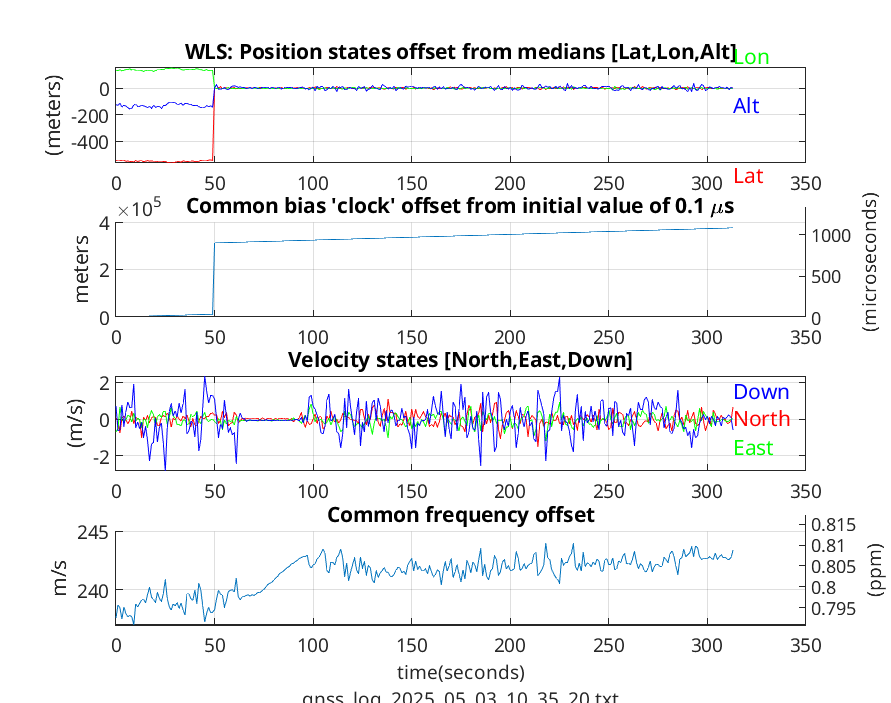
\includegraphics[width=\textwidth]{images/tests/Monte_Cappuccini/Spoofing/task6_figures/Samsung_A51_Monte_Cappuccini_fig5.png}
                \caption{Delay: WLS states and bias}
            \end{subfigure}
            \hfill
            \begin{subfigure}{0.23\textwidth}
                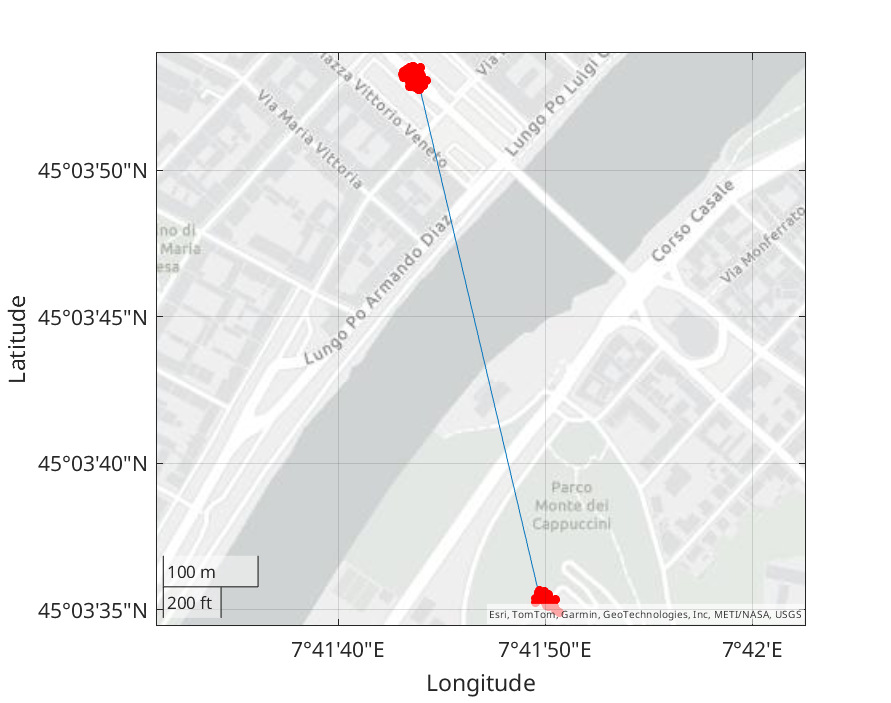
\includegraphics[width=\textwidth]{images/tests/Monte_Cappuccini/Spoofing/task6_figures/Samsung_A51_Monte_Cappuccini_fig6.png}
                \caption{Delay: Position}
            \end{subfigure}
        \end{figure}

        \noindent As visible in the plots, all observables remain nominal until t=50 s, at which point the solver's estimated position and receiver clock-bias exhibit a clear discontinuity as the spoof takes effect.

        \begin{itemize}
            \item \textbf{Position solution:} Prior to 50 s, the estimated coordinate coincides with the true static point. Immediately after 50 s, the solution jumps to the spoofed Piazza Vittorio Veneto location, replicating the static-spoof offset of several hundred metres.  
            \item \textbf{Receiver clock-bias:} A sudden step of appears in the estimated receiver clock-bias track, directly corresponding to the 1 ms replay delay needed to shift the range solution by the planar offset.  
            \item \textbf{Carrier-to-noise density (C/N):} The C/N time-series shows no amplitude change at t=50 s—signal strength is unaffected by delay.  
            \item \textbf{Dilution of precision (PDOP):} Satellite geometry quality remains continuous and invariant through the spoof onset.  
            \item \textbf{Pseudorange residuals:} Residuals maintain the same spread, but their mean shifts abruptly at 50 s by the additional delay delta t.  
        \end{itemize}
        
        \noindent From a solver-stability perspective, the sudden time bias causes an immediate step in both position and clock-bias, sometimes triggering a brief convergence glitch (extra iterations or loss of fix) as the estimator re-optimizes. 
        Even a 1 ms replay delay can therefore introduce a large positional error and matching clock-bias shift without altering any standard observables. Detecting such covert delay-based spoofing thus requires monitoring for timing discontinuities.

    \subsection{Interference Effects}
    
        % If performed, explain signal degradations, cycle slips, and accuracy loss

        % content
